% Long: they only share an instruction when it is the same. They do not do
% anything to synchronize the threads.

% 

\documentclass[times,10pt,twocolumn]{article} 

\usepackage{tikz}
\usepackage{caption}
\usepackage{amsfonts}
\usepackage{enumitem}
\usepackage{subcaption}
%\usepackage[lined,ruled,linesnumbered]{algorithm2e}

\usepackage{amsmath,amssymb}
\usepackage{fullpage}
\usepackage{graphicx}
\usepackage{setspace}
\usepackage{stmaryrd}
%\usepackage{proof}
\usepackage{skak} % for the \qside
\usepackage{array}
\usepackage{url}

\usetikzlibrary{positioning,shapes.geometric}
\usetikzlibrary{arrows}
\usetikzlibrary{automata}

\newtheorem{theorem}{Theorem}[section]
\newtheorem{corollary}[theorem]{Corollary}
\newtheorem{definition}[theorem]{Definition}

\newcommand{\tid}{\mbox{\texttt{T}}_{id}}
\newcommand{\simd}{$\mu$-\textsc{Simd}}
\newcommand{\code}[1]{\mbox{\texttt{#1}}}

\begin{document}

\title{Function Call Fusion
\thanks{This work was partially supported by CNPq, CAPES, FAPEMIG.}
}

\author{Douglas do Couto Teixeira ~~ Sylvain Collange ~~ Fernando Magno Quint\~{a}o Pereira\\
Departamento de Ci\^{e}ncia da Computa\c{c}\~{a}o ~~
Universidade Federal de Minas Gerais, Brazil\\
{\small {\tt \{douglas,sylvain.collange,fernando\}@dcc.ufmg.br}}
} 

\maketitle
\thispagestyle{empty}

\maketitle

\begin{abstract}
% Context
The increasing popularity of Graphics Processing Units (GPUs), has brought
renewed attention to old problems related to the Single Instruction, Multiple
Data execution model.
% Problem
One of these problems is the reconvergence of divergent threads.
A divergence happens at a conditional branch when different threads that reach
it in lock-step disagree on the path to follow.
Divergences are common in general purpose applications, and may impose a heavy
burden on the performance of parallel programs.
% Solution
In this paper we propose a compiler-level optimization to mitigate the loss of
performance due to divergences.
This optimization consists in merging function call sites located at different
paths that sprout from the same branch.
% Results
We show that our optimization adds negligible overhead on the compiler.
It does not slowdown programs in which it is not applicable, and accelerates
substantially those in which it is.
As an example, we have been able to speed up the well known SPLASH Fast Fourier
Transform benchmark by XX\%.
\end{abstract}

%%%%%%%%%%%%%%%%%%%%%%%%%%%%%%%%%%%%%%%%%%%%%%%%%%%%%%%%%%%%%%%%%%%%%%%%%%%%%%%%

\section{Introduction}
\label{sec:int}

% Context:
Graphics Processing Units (GPUs) are becoming a staple hardware in the
high-performance world.
They provide a simple, cheap, and efficient platform in which parallel
applications can be developed~\cite{Nickolls10}.
Since the release of CUDA, in early 2006~\cite{Garland08}, a plethora
of programming patterns and algorithms have been designed to run in this
environment.
Applications that run on Graphics Processing Units constitute, today, a diverse
group.
They solve problems as different as gene sequencing~\cite{Sandes10},
IP routing~\cite{Mu10}, linear algebra~\cite{Zhang10} and program
analysis~\cite{Prabhu11}.
% TODO: you must back off these claims with citations.

% Problem:
Nevertheless, in spite of all these advances, programming applications for
GPUs remains a challenging task.
One of the reasons behind this difficulty is a phenomenon known as
{\em Thread Divergence}.
When facing a conditional branch, two threads diverge if 
they disagree on which path to take.
Divergences are a problem because they have an impact on the program's
performance.
In other words, a divergence splits threads into two groups, upon reaching a
conditional branch.
Only one of these groups contain threads that do useful work at a given point
in time.

% Solution:
We have designed, implemented and tested a compiler optimization that
mitigates this performance loss.
We name this optimization {\em Fusion of Calling Sites}.
Our optimization relies on a simple idea: threads should enter functions
in lock-step to minimize the effects of divergences.
Therefore, whenever a function is invoked at the two different paths that stem
from a conditional test, we merge the two calling sites into one single
invocation of that function.

% Result:
As we show in Section~\ref{sec:sol}, our algorithm scans blocks of code within
the program, performing the merging whenever it is possible.
In Section~\ref{sec:ovf}, we demonstrate that our optimization is:
(i) easy to implement, (ii) innocuous when non-applicable and
(iii) effective when used.
Our implementation is relatively simple, and it has low computational
complexity.
In other words, our optimization always applies a constant number of
operations per pair of calling sites that it merges.
If a program does not present any opportunity for this merging to happen,
then we do not impose any runtime overhead onto the compiler, nor onto the
executable program, once it is deployed.
In Section~\ref{sec:exp}, we show the potential of our optimization through a
toy benchmark, and show its applicability in the well-known implementation of
Fast Fourier Transform available in SPLASH\footnote{\url{http://www.capsl.udel.edu/splash/}}.

\section{Overview of the Approach}
\label{sec:ovf}

\begin{figure}[b!]
\begin{center}

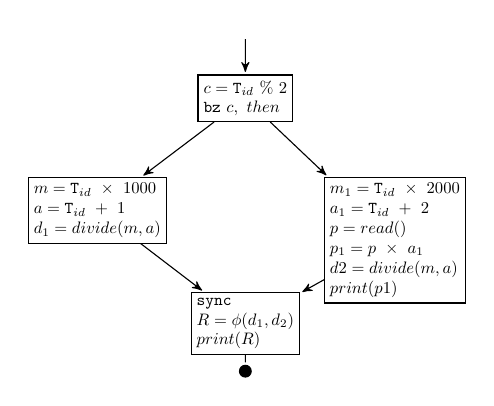
\begin{tikzpicture}
\tikzset{
    every node/.style = {draw, rectangle, scale=.60, auto, align=left},
    every path/.style = {draw, >=stealth', shorten >=1pt, auto},
    snake/.style = {decorate, decoration=snake},
    baseline = (current bounding box.north)
}

% -------------------------------------------------------
\node[draw=none] (0) {};

\node[below=15pt] (entry) at (0) {
    $c = \tid \ \% \ 2$ \\
    $\code{bz} \ c, \  then$
};

\node[below left=of entry] (then) at (entry) {
    $m = \tid \ \times \ 1000$ \\
    $a = \tid \ + \ 1$ \\
    $d_{1} = divide(m, a)$
};

\node[below right=of entry] (else) at (entry) {
    $m_{1} = \tid \ \times \ 2000$ \\
    $a_{1} = \tid \ + \ 2$ \\
    $p = read()$ \\
    $p_{1} = p \ \times \ a_{1}$ \\
    $d{2} = divide(m, a)$ \\
    $print(p1)$
};

\node[below=70pt] (end) at (entry) {
    $\code{sync}$ \\
    $R = \phi(d_{1}, d_{2})$ \\
    $print(R)$
};

\node[below=15pt, fill=black, circle, scale=.75] (e) at (end) {};

% -------------------------------------------------------
\path[->] (0) edge (entry);

\path[->] (entry) edge (then);
\path[->] (entry) edge (else);

\path[->] (then) edge (end);
\path[->] (else) edge (end);

\path[-] (end) edge (e);
\end{tikzpicture}

\caption{}
\label{code-b}

\begin{small}
\begin{tabular}{|c|l|c|c|c|c|} \hline
Cycle   & Instruction                  & $t_0$        & $t_1$        & $t_2$        & $t_3$        \\ \hline
14      & $ c = \tid \% 2$             & $\checkmark$ & $\checkmark$ & $\checkmark$ & $\checkmark$ \\ \hline
15      & $ \code{bz} \ c, then$ & $\checkmark$ & $\checkmark$ & $\checkmark$ & $\checkmark$ \\ \hline
16      & $ m = \tid \ \times \ 1000$        & $\checkmark$    & $\bullet$ & $\checkmark$ & $\bullet$ \\ \hline
17      & $ a = \tid \ + \ 1$ & $\checkmark$    & $\bullet$ & $\checkmark$ & $\bullet$ \\ \hline
18      & $ d1 = divide(m, a)$ & $\checkmark$    & $\bullet$ & $\checkmark$ & $\bullet$ \\ \hline
\multicolumn{6}{c}{$\ldots$} \\ \hline
118      & $ m1 = \tid \ \times 2000$ & $\bullet$    & $\checkmark$ & $\bullet$ & $\checkmark$ \\ \hline
119     & $ a1 = \tid \ + \ 2$        & $\bullet$    & $\checkmark$    & $\bullet$ & $\checkmark$ \\ \hline
120     & $ p = read()$ & $\bullet$    & $\checkmark$    & $\bullet$ & $\checkmark$ \\ \hline
121     & $ p1 = p \ \times a1$ & $\bullet$    & $\checkmark$ & $\bullet$ & $\checkmark$ \\ \hline
122     & $ d2 = divide(m, a)$        & $\bullet$    & $\checkmark$    & $\bullet$ & $\checkmark$ \\ \hline
\multicolumn{6}{c}{$\ldots$} \\ \hline
222      & $ print(p1)$ & $\bullet$    & $\checkmark$    & $\bullet$ & $\checkmark$ \\ \hline
223     & $ \code{sync}$        & $\checkmark$ & $\checkmark$ & $\checkmark$ & $\checkmark$ \\ \hline
224     & $ R = phi(d1, d2)$    & $\checkmark$ & $\checkmark$ & $\checkmark$ & $\checkmark$ \\ \hline
225     & $ print(R)$ & $\checkmark$    & $\checkmark$ & $\checkmark$ & $\checkmark$ \\ \hline
\end{tabular}

\end{small}
\end{center}
\caption{(Top) A program whose performance may experience a slowdown due to divergences.
% TODO: add arrows to the edges in the CFG. Make these edges shorter.
% TODO: The figure is taking more space than necessary.
% TODO: Replace the phi-function with a sync instruction in the figure.
% you have not explained what is SSA, and maybe you can write the paper
% without having to explain this.
(Bottom) An execution trace of the program.
If a thread $t$ executes an instruction at cycle
$j$, we mark the entry $(t, j)$ with $\checkmark$.
Otherwise, we mark it with $\bullet$.
In this example we assume that function \texttt{divide} takes one hundred
cycles to execute.}
\label{fig:exampleOrig}
\end{figure}

Figure~\ref{fig:exampleOrig} will let us illustrate thread divergences.
This phenomenon characterizes the Single Instruction, Multiple Data
execution model typical of Graphics Processing Units.
These processors organize threads in groups that execute in lock-step.
Such groups are called {\em warps} in NVIDIA's jargon, or {\em wavefronts} in
AMD's.
We can imagine that threads in the same warp use different arithmetic and
logic units, but share the same instruction control logic.
Control flow divergences happen when threads
in a warp follow different paths after processing the same branch.
If the branching condition is data divergent, then it might be true to some
threads, and false to others.
In face of divergences, some threads will take the ``then" part of the branch
in Figure~\ref{fig:exampleOrig}, and others will take the ``else" part.
Due to our restriction of sharing the instruction control logic, only one group
of threads will be allowed to do useful work at a given instant.
The execution trace at the bottom of Figure~\ref{fig:exampleOrig} shows
which threads are active at each cycle, assuming an architecture that allows
four threads simultaneously in flight.

When two threads diverge, the hardware should reconverge them as earlier as
possible to maximize the amount of active workers per cycles.
A {\em reconvergence point} is the earliest instruction in the program where we
can expect program paths to reconverge  regardless of the outcome or target of
the divergent branch.
Fung {\em et al.} have shown that the {\em post-dominator} of a branch is --
usually -- the best place to reconverge threads~\cite{Fung07}.
We say that a node $v$ in a CFG post-dominates a node $u$ if any path from $v$
to the end of the CFG must go across $u$.
In Figure~\ref{fig:exampleOrig}, basic block \texttt{end} is the post-dominator
of every other block.
Yet, as Fung {\em et al.} themselves have also showed, reconverging threads at the
post-dominators of branches is far from being a perfect solution to divergences.
Figure~\ref{fig:exampleOrig} illustrates this situation particularly well.

The \texttt{divide} function is invoked at both sides of the branch in
Figure~\ref{fig:exampleOrig}.
Even though this function must be executed by all the threads that reach the
divergent branch, these threads will be entering the function at different
execution cycles due to the divergence.
Consequently, the instructions that constitute function \texttt{divide} will
be called twice: once for the threads in the ``then" part of the branch, and
another time for the threads in the ``else" part.
In this case, reconverging threads at post-dominators of divergent points will
not avoid the redundant execution of \texttt{divide}.
If \texttt{divide} runs for a long time, then we will be missing the
opportunity to share many execution cycles among different threads.
The goal of function call fusion is to reconverge threads at the entry points
of functions.
We will accomplish this goal by changing the structure of the program's
control flow graph, as we will explain in the next section.

\section{Fusion of Calling Sites}
\label{sec:sol}

In this section we will give a detailed explanation of our optimization. 
We will use the program from Figure~\ref{fig:exampleOrig} as our running
example.
In that program, our goal is to combine both invocations of the ``divide''
function.
In Figure~\ref{fig:exampleOpt} we show the same program seen in 
Figure~\ref{fig:exampleOrig} after our optimization.
As we can see from Figure~\ref{fig:exampleOrig} and Figure~\ref{fig:exampleOpt},
our optimization is able to slightly reduce divergences.
In the following sections we will explain how our optimization works in details
and how we are able to reduce such divergences.
sections
% Figure showing the program optimized.


\begin{figure}[htb]
\begin{center}
%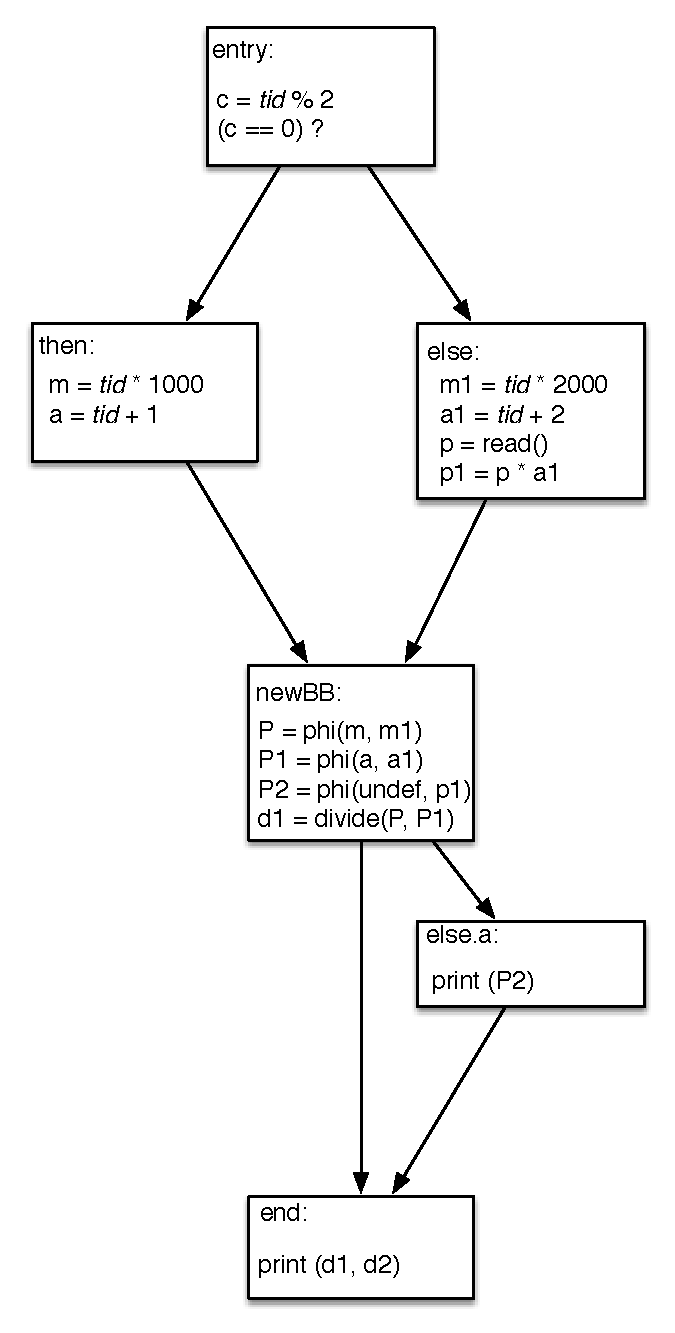
\includegraphics[scale=0.5]{images/exampleOpt}

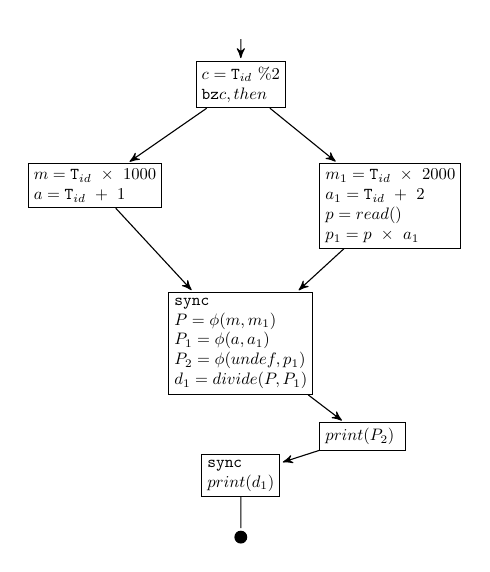
\begin{tikzpicture}
\tikzset{
    every node/.style = {draw, rectangle, scale=.60, auto, align=left},
    every path/.style = {draw, >=stealth', shorten >=1pt, auto},
    snake/.style = {decorate, decoration=snake},
    baseline = (current bounding box.north)
}

% -------------------------------------------------------
\node[draw=none] (0) {};

\node[below=10pt] (entry) at (0) {
    $c = \tid \ \% 2$ \\
    $\code{bz} c, then$
};

\node[below left=of entry] (then) at (entry) {
    $m = \tid \ \times \ 1000$ \\
    $a = \tid \ + \ 1$    
};

\node[below right=of entry] (else) at (entry) {
    $m_{1} = \tid \ \times \ 2000$ \\
    $a_{1} = \tid \ + \ 2$ \\
    $p = read()$ \\
    $p_{1} = p \ \times \ a_{1}$
};

\node[below=75pt] (newBB) at (entry) {
    $\code{sync}$ \\
    $P = \phi(m, m_{1})$ \\
    $P_{1} = \phi(a, a_{1})$ \\
    $P_{2} = \phi(undef, p_{1})$ \\
    $d_{1} = divide(P, P_{1})$
};


\node[below right=of newBB] (elsea) at (newBB) {
    $print(P_{2})$
};

\node[below=40pt] (end) at (newBB) {
    $\code{sync}$ \\
    $print(d_{1})$
};

\node[below=20pt, fill=black, circle, scale=.75] (e) at (end) {};

% -------------------------------------------------------
\path[->] (0) edge (entry);

\path[->] (entry) edge (then);
\path[->] (entry) edge (else);

\path[->] (then) edge (newBB);
\path[->] (else) edge (newBB);
\path[->] (newBB) edge (elsea);
\path[->] (elsea) edge (end);

\path[-] (end) edge (e);
\end{tikzpicture}

\caption{}
\label{code-b}


% TODO: make this function smaller (make edges shorter).
\begin{small}
\begin{tabular}{|c|l|c|c|c|c|} \hline
Cycle   & Instruction                  & $t_0$        & $t_1$        & $t_2$        & $t_3$        \\ \hline
14      & $ c = \tid \% 2$             & $\checkmark$ & $\checkmark$ & $\checkmark$ & $\checkmark$ \\ \hline
15      & $ \code{bz} \ c, then$ & $\checkmark$ & $\checkmark$ & $\checkmark$ & $\checkmark$ \\ \hline
\multicolumn{6}{c}{$\ldots$} \\ \hline
16      & $ m = \tid \ \times \ 1000$        & $\checkmark$    & $\bullet$ & $\checkmark$ & $\bullet$ \\ \hline
17      & $ a = \tid \ + \ 1$ & $\checkmark$    & $\bullet$ & $\checkmark$ & $\bullet$ \\ \hline
\multicolumn{6}{c}{$\ldots$} \\ \hline
25      & $ m1 = \tid \ \times 2000$ & $\bullet$    & $\checkmark$ & $\bullet$ & $\checkmark$ \\ \hline
26      & $ a1 = \tid \ + \ 2$        & $\bullet$    & $\checkmark$    & $\bullet$ & $\checkmark$ \\ \hline
27      & $ p = read()$ & $\bullet$    & $\checkmark$    & $\bullet$ & $\checkmark$ \\ \hline
28      & $ p1 = p \ \times \ a1$ & $\bullet$    & $\checkmark$    & $\bullet$ & $\checkmark$ \\ \hline
\multicolumn{6}{c}{$\ldots$} \\ \hline
45      & $ \code{sync}$        & $\checkmark$ & $\checkmark$ & $\checkmark$ & $\checkmark$ \\ \hline
46      & $ P = phi(m, m1)$    & $\checkmark$ & $\checkmark$ & $\checkmark$ & $\checkmark$ \\ \hline
47      & $ P2 = phi(P, P1)$ & $\checkmark$    & $\checkmark$ & $\checkmark$ & $\checkmark$ \\ \hline
48      & $ d1 = divide(P, P1)$ & $\checkmark$    & $\checkmark$ & $\checkmark$ & $\checkmark$ \\ \hline
\multicolumn{6}{c}{$\ldots$} \\ \hline
49      & $ print(P2)$ & $\bullet$    & $\checkmark$ & $\bullet$ & $\checkmark$ \\ \hline
\multicolumn{6}{c}{$\ldots$} \\ \hline
51      & $ \code{sync}$        & $\checkmark$ & $\checkmark$ & $\checkmark$ & $\checkmark$ \\ \hline
52      & $ print(d1)$ & $\checkmark$    & $\checkmark$ & $\checkmark$ & $\checkmark$ \\ \hline
\end{tabular}

\end{small}
\end{center}
\caption{(Top) The same program from Figure~\ref{fig:exampleOrig} after being optimized.
(Bottom) An execution trace of the program.
If a thread $t$ executes an instruction at cycle
$j$, we mark the entry $(t, j)$ with the symbol $\checkmark$.
Otherwise, we mark it with $\bullet$.}
\label{fig:exampleOpt}
\end{figure}

% TODO: this explanation is confusing, and, again, I think it is better not
% to talk about SSA form.
One of the main difficulties in implementing our optimization concerns the
correct usage of function arguments.
We do not know beforehand which parameters
will be passed to the function at running time.
Thus, even if, at the source code level, the two calls of the function receive
the same variable name as parameter, when the code is transformed to SSA, the 
function will see different variable names.
Therefore, we need a strategy to not only merge functions but also to combine 
the parameters, in such a way that the function will always receive the right
ones at running time.

The SSA form brings up the problem of passing different variables as parameters
to the function, but it also provides a solution. 
% TODO: which solution? This first sentence has no connection with the rest
% of the text.
We solve this problem by creating a basic block to host the new call of the 
function as well as its combined parameters. 
If we break down the procedure used to generate the program shown in 
Figure~\ref{fig:exampleOpt} we will notice that: i) both the ``then'' and
the ``else'' blocks were split into two new blocks each; ii) the original
calls to ``divide'' were removed; iii) a new block was created to acomodate
the new call to ``divide'' along with \textit{Phi} nodes to combine the
parameters; iv) the original condition of the branch was inserted into the
new block.

% Describe the problems, mainly, the dominance one
% TODO: replace phi functions with selectors. Let's not talk about SSA form?
The use of \textit{Phi} functions solves the problem of combining the 
parameters, but yet another problem arises: by inserting a new block into the 
function, we break the dominance tree. 
% TODO: know your audience. Readers may not know what is a dominance tree.
More specifically, the instruction ``p1''
does not dominate the call to ``print'' in the ``else.a'' block. 
% TODO: and why is this a problem? You are assuming that the reader knows
% too much.
We notice, however, that whenever the control flow reaches the ``else'' block,
it will also reach ``else.a'' because the branch condition in ``newBB'' is the
same as the one in ``entry''. 
This fact allows us to place a \textit{Phi} function with an \textit{undef} 
parameter into ``newBB'', making sure that ``p1'' now dominates 
``else.a'', and the branch condition assures that the \textit{undef} parameter
will never be used.


% Explain how the algorith works by traversing the blocks
% TODO: what is the algorithm? Could you write it in pseudo-code?
Merging calling sites is an involved procedure, but we shall show that our 
algorithm terminates, and that it is correct, i.e., it preserves the  program's
semantic.
As we described before, most of the operations our algorithm executes have 
constant asymptotic complexity. 
We have, however, to analyze every branch of the function to check whether or
not it contains function calls that can be merged. The asymptotic complexity
of this procedure is linear in the number of basic blocks in the function. 
The algorithm terminates because we optimize a basic block only once. 
And it is is correct because by using \textit{Phi} functions to merge 
parameters we guarantee that, at running time, only the correct ones will be
passed to the function.
% TODO: that is not a proof of correctness.

\section{Experimental Results}
\label{sec:exp}

Our optimization is meant to be executed in SIMD hardware with explicit
synchronization.
In this model, each thread keeps its own program counter (PC) and at fetch 
time, the hardware chooses heuristically the next PC to serve to the threads.
If the chosen PC is the same across several threads, then these threads execute
the same instruction.
If the input values are the same for all threads executing the instruction,
then the computations are combined too, so the instruction is issued once
on behalf of all participating threads.
It is a theoretical model, but it can be implemented as a MIMD machine that is
able to share fetch and decode units while other units are unused.

There are several heuristics to choose which PC to to serve, but no hardware to 
implement them all.
To solve this problem we built a framework to simulate the heuristics.
Our framework uses LLVM to compile the source code and merge calling sites.

To evaluate our optimization, we use a trace-driven idealized architecture simulator
implemented as a Pin tool~[REF PIN].
Our Pin tool reads the binary and produces traces representing every 
instruction that each thread executes. 
Then, we replay the traces inside the simulator and measure our 
optimization's results.

Our framework simulates three heuristics: MinSP-PC, MaxFun-MinPC, and Long-MinSP-PC.
The heuristic called MinSP-PC was proposed by Collange [CITATION] and is 
built on top of Quinn's Min-PC heuristic[CITATION].
It is used in programs that contain function invocations.
The bedrock of MinSP-PC is the fact that when a function is called, the stack
grows down.
Thus, threads running more deeply nested function calls have smaller SPs.
This heuristic chooses, then, those threads with the smallest SP, because it
assumes that those threads will need more processing time.
MaxFun-MinPC (Maximum Function Level - Minimum PC) is much like MinSP-MinPC,
but instead of choosing the smallest SP, it chooses the thread that has the the
highest number of activation records on the stack.
Therefore, this heuristic would have the same behavior of MinSP-MinPC if all
activation records had the same size. 
Long [CITATION] created a heuristic to analyse redundancies in SIMD programs.
Its key idea is to add some sort of memory to each thread.
One thread uses the memory of the others to advance or stall.
If the current PC of a thread $t_{0}$ is in the recent history of another
thread $t_{1}$, then thread $t_{0}$ is probably behind $t_{1}$.
In this case, $t_{0}$ needs to progress to catch up with $t_{1}$.
The idea of Long’s heuristic can be used to create other heuristics.
When multiple threads have the same highest priority, the original heuristic
executes these threads alternately, but the variations of Long's heuristic use
other policies to choose the next thread to execute.
In this paper we used Long's with Min-PC: when multiple threads have the
highest priority, the basic block of the threads with smallest PC is executed
first.
Then, all priorities are recounted again for the next choice.

We show the effectiveness of our optimization in the Fast 
Fourier Transform (FFT) benchmark, taken from SPLASH2X benchmark, in the
PARSEC benchmark[CITATION] suite.
We show that our optimization increases the
instruction share rate in all three heuristics in the FFT benchmarks.

%FFT
%2 threads
%Heuristic;LLVM;LLVM+Opt
%Long-MinSP-PC;1,0645300;1,0311560
%MaxFun-MinPC (3)    1,0645300   1,0311570
%MinSP-PC    1,0645300   1,0311570
%4 threads
%Long-MinSP-PC (8)   1,0948930   1,0468920
%MaxFun-MinPC (3)    1,0948920   1,0468920
%MinSP-PC    1,0948920   1,0468910
%8 threads
%Long-MinPC (8)  5,5348080   5,5336100
%MaxFun-MinPC (3)    1,1105330   1,0549930
%MinSP-PC    1,1105330   1,0549930
%16 threads
%Long-MinSP-PC (8)   1,1192670   1,0595030
%MaxFun-MinPC (3)    1,1192640   1,0595040
%MinSP-PC    1,1192640   1,0595040

% TODO: show results for the toy benchmark.

Furthermore, we show that our optimization reduces the number of instructions
dynamically executed in the program.
We performed this experiment by running our program through a Pin tool that logs
every instruction executed by each thread. Table [REF] shows the results.

% bench      2 threads 4 threads ....
%fft         2641    3295    3297    4002    4023    17258  100\%
%fft + Opt   2641    3287    3279    3265    3250    15722  91,1\%

We ran the experiments in a machine running Ubuntu 12.04 (Kernel version 3.2.0), with 16 GB of DDR2 RAM, and a Intel Xeon CPU E5-2620 2.00GHz processor.

\section{Related Work}
\label{sec:rw}

\begin{itemize}
\item Works on Divergence Optimisations (See the paper: ``Divergence Analysis")
\item Works on reconvergence heuristics (See the paper: ``Simultaneous branch and warp interweaving for sustained GPU performance")
Collange, S. (2011). Stack-less SIMT reconvergence at low cost. Technical report, ENS Lyon.
\end{itemize}

\section{Conclusion}
\label{sec:con}

\bibliographystyle{IEEEtran}
\bibliography{references}

\end{document}
